\documentclass[a4paper,12pt]{article}

% 基础宏包
\usepackage[UTF8]{ctex}
\usepackage{geometry}
\usepackage{graphicx}
\usepackage{booktabs}
\usepackage{hyperref}
\usepackage{amsmath}
\usepackage{amsfonts}
\usepackage{amssymb}
\usepackage{float}
\usepackage{subcaption}
\usepackage{multirow}
\usepackage{array}
\usepackage{xcolor}

% 页面设置
\geometry{left=2.5cm, right=2.5cm, top=3cm, bottom=3cm}

% 超链接设置
\hypersetup{
    colorlinks=true,
    linkcolor=blue,
    filecolor=magenta,      
    urlcolor=cyan,
    citecolor=blue,
}

% 标题信息
\title{\textbf{\huge ABM 仿真系统实验分析报告}\\[0.5cm]
\Large 基于 Ising-D-I-B 模型的消费者行为与 AI 代理研究}
\author{ABM 研究团队}
\date{\today}

\begin{document}

\maketitle

\begin{abstract}
\noindent 本报告系统地分析了基于 Ising-D-I-B 耦合模型的多智能体（ABM）仿真实验结果。研究通过基线模型和五个专项实验，深入探讨了消费者在 AI 代理辅助下的决策行为演化机制。实验涵盖了记忆机制、AI 进化、信息干预、语境敏感性和过滤气泡、系统性风险等关键问题。研究发现：社会影响强度达到临界值时会出现相变现象，导致消费者向高度依赖型集中；记忆机制能够有效降低错误率但可能抑制创新探索；适度的信息干预可以优化系统性能；语境敏感性显著影响决策质量；过滤气泡效应可能导致群体极化；系统性风险在网络中具有快速传播特性。这些发现为理解人机协同决策系统提供了重要的理论依据和实践指导。

\vspace{1cm}
\noindent \textbf{关键词}：多智能体仿真；Ising 模型；D-I-B 框架；消费者行为；AI 代理；社会网络；相变；集体涌现
\end{abstract}

\tableofcontents
\newpage

\section{引言}

\subsection{研究背景}

随着人工智能技术的快速发展，AI 代理系统在金融投资、医疗诊断、教育辅导等领域得到广泛应用。然而，人类对 AI 的依赖程度及其社会影响机制仍不清楚。特别是在社交网络环境下，个体间的相互影响如何与 AI 代理系统相互作用，进而影响集体行为模式，这是一个亟待解决的科学问题。

\subsection{理论基础}

本研究整合了三个核心理论框架：

\begin{enumerate}
    \item \textbf{Ising 模型}：源自统计物理学，用于描述磁性材料的相变现象。在本研究中用于模拟社交网络中的社会影响传播和集体行为涌现。
    
    \item \textbf{D-I-B 框架}（Dependency-Information-Behavior）：消费者行为学理论，将消费者对 AI 的依赖程度分为五个等级：L1 自主型、L2 信息辅助型、L3 半委托型、L4 高度依赖型、L5 完全代理型。
    
    \item \textbf{复杂适应系统理论}：强调系统的涌现性、自组织性和非线性特征，为理解微观个体行为与宏观集体现象的关系提供了理论指导。
\end{enumerate}

\subsection{研究目标}

本研究的主要目标包括：
\begin{itemize}
    \item 构建整合 Ising 社会网络和 D-I-B 消费者的 ABM 仿真平台
    \item 揭示社会影响强度对集体依赖模式的相变机制
    \item 探究记忆学习、AI 进化、信息干预等因素的调节作用
    \item 识别系统性风险的传播规律和韧性特征
    \item 为 AI 治理和人机协同优化提供政策建议
\end{itemize}

\section{总体研究方法}

\subsection{模型架构}

本研究的 ABM 仿真系统包含四个核心组件：

\subsubsection{Ising 社交网络}

采用自适应 Ising 网络模拟消费者间的社会影响：
\begin{equation}
    H = -J \sum_{\langle i,j \rangle} s_i s_j - h \sum_i s_i
\end{equation}
其中 $s_i \in \{-1, +1\}$ 表示个体 $i$ 的状态，$J$ 为耦合强度（社会影响强度），$h$ 为外部场（媒体影响）。

\subsubsection{D-I-B 消费者智能体}

每个消费者具有以下特征：
\begin{itemize}
    \item \textbf{依赖等级} $L \in \{1,2,3,4,5\}$：对应自主型到完全代理型
    \item \textbf{信任度} $\tau \in [0,1]$：对 AI 的信任程度
    \item \textbf{满意度} $S \in [0,1]$：决策后的主观效用评价
    \item \textbf{记忆容量} $M$：可存储的历史经验数量（实验 2 特有）
\end{itemize}

\subsubsection{AI 代理群体}

AI 代理系统包含以下特征：
\begin{itemize}
    \item \textbf{能力参数} $\alpha \in [0,1]$：决策准确性
    \item \textbf{错误率} $\epsilon \in [0,1]$：犯错概率
    \item \textbf{进化能力}：通过强化学习优化策略（实验 3）
\end{itemize}

\subsubsection{市场环境}

模拟包含以下要素：
\begin{itemize}
    \item \textbf{产品类别}：高质量/低质量产品
    \item \textbf{决策任务}：二选一消费选择
    \item \textbf{反馈机制}：基于产品质量的满意度更新
\end{itemize}

\subsection{仿真流程}

每个仿真步包含以下步骤：
\begin{enumerate}
    \item Ising 网络更新：根据 Metropolis 准则更新个体状态
    \item 依赖等级调整：基于满意度和信任度更新 $L$
    \item AI 使用决策：高等级个体调用 AI 代理
    \item 环境交互：执行决策并获得反馈
    \item 指标记录：统计宏观系统指标
\end{enumerate}

\subsection{实验设计原则}

所有实验遵循以下设计原则：
\begin{itemize}
    \item \textbf{对照原则}：设置基线组作为参照
    \item \textbf{单一变量}：每次仅改变一个关键参数
    \item \textbf{重复验证}：多次运行确保结果稳健性
    \item \textbf{多指标评估}：从多个维度量化系统行为
\end{itemize}

\section{实验 1：基线模型——Ising-D-I-B 耦合机制验证}

\subsection{研究问题}

基线实验旨在回答以下核心问题：
\begin{enumerate}
    \item Ising 社会影响机制能否有效耦合到消费者决策框架中？
    \item 系统是否会出现预期的相变现象（向 L4 高度依赖型集中）？
    \item 磁化强度与依赖等级分布之间存在何种关联？
    \item 小世界网络拓扑结构如何影响传播动力学？
\end{enumerate}

\subsection{研究方法}

\subsubsection{实验设计}

\begin{table}[H]
\centering
\caption{基线实验参数配置}
\begin{tabular}{lll}
\toprule
\textbf{参数类型} & \textbf{符号} & \textbf{取值} \\
\midrule
消费者数量 & $N$ & 500 \\
AI 代理数量 & $n_{AI}$ & 3 \\
初始耦合强度 & $J_0$ & 0.05 \\
温度 & $T$ & 1.0 \\
仿真步数 & $Steps$ & 100 \\
WS 网络重连概率 & $p$ & 0.3 \\
平均度数 & $\langle k \rangle$ & 6 \\
\bottomrule
\end{tabular}
\end{table}

\subsubsection{初始条件}

依赖等级初始分布设置为正态分布：
\begin{equation}
    P(L) \sim \mathcal{N}(\mu=3, \sigma=1)
\end{equation}
具体分布为：L1: 50 人，L2: 125 人，L3: 150 人，L4: 125 人，L5: 50 人。

\subsubsection{观测指标}

\textbf{宏观指标}：
\begin{itemize}
    \item 磁化强度 $M(t) = \frac{1}{N}\sum_i s_i$
    \item 耦合强度演化 $J(t)$
    \item 磁化率 $\chi = \frac{\partial M}{\partial h}$
\end{itemize}

\textbf{微观指标}：
\begin{itemize}
    \item 依赖等级分布 $P(L,t)$
    \item 平均满意度 $\bar{S}(t)$
    \item AI 使用率 $R_{AI}(t)$
    \item 错误率 $\epsilon(t)$
\end{itemize}

\textbf{网络指标}：
\begin{itemize}
    \item 平均聚类系数 $C$
    \item 平均路径长度 $d$
    \item 度分布 $P(k)$
\end{itemize}

\subsection{结果分析}

\subsubsection{依赖等级演化}

实验结果显示，系统呈现明显的演化趋势：
\begin{itemize}
    \item \textbf{L1 自主型}：从 50 人降至 0 人（$\Delta = -50$）
    \item \textbf{L2 信息辅助型}：从 125 人降至 53 人（$\Delta = -72$）
    \item \textbf{L3 半委托型}：从 150 人降至 88 人（$\Delta = -62$）
    \item \textbf{L4 高度依赖型}：从 125 人激增至 359 人（$\Delta = +234$）$\star$
    \item \textbf{L5 完全代理型}：从 50 人降至 0 人（$\Delta = -50$）
\end{itemize}

\textbf{关键发现}：系统出现了显著的"向 L4 集中"现象，验证了相变假说。

\subsubsection{Ising 动力学特征}

磁化强度演化显示：
\begin{equation}
    M: 0.012 \rightarrow 0.306 \quad (\text{变化量 } \Delta M = +0.294)
\end{equation}

耦合强度演化特征：
\begin{itemize}
    \item 初期缓慢增长：$J: 0.05 \rightarrow 0.12$（前 30 步）
    \item 中期加速上升：$J: 0.12 \rightarrow 0.28$（30-70 步）
    \item 后期趋于饱和：$J \approx 0.30$（70 步后）
\end{itemize}

\textbf{物理解释}：当耦合强度超过临界值 $J_c \approx 0.1667$ 时，系统发生二级相变，从无序态（各等级均匀分布）转变为有序态（L4 主导）。

\subsubsection{系统性能分析}

\begin{table}[H]
\centering
\caption{基线模型性能指标统计}
\begin{tabular}{lll}
\toprule
\textbf{指标} & \textbf{均值} & \textbf{标准差} \\
\midrule
平均满意度 & 0.437 & 0.082 \\
AI 使用率 & 0.838 & 0.045 \\
错误率 & 0.082 & 0.023 \\
\bottomrule
\end{tabular}
\end{table}

满意度演化呈现先降后升的趋势，表明系统在经历相变后达到新的平衡态。

\subsubsection{网络拓扑特征}

小世界网络分析结果：
\begin{itemize}
    \item 平均聚类系数：$C = 0.197$
    \item 平均路径长度：$d = 4.10$
    \item 小世界系数：$\sigma = \frac{C/C_{rand}}{d/d_{rand}} > 1$
\end{itemize}

这表明 WS 网络成功构建了小世界特性，有利于社会影响的快速传播。

\subsection{本节小结}

基线实验成功验证了 Ising-D-I-B 耦合模型的有效性：
\begin{enumerate}
    \item[$\checkmark$] Ising 机制能够成功整合到消费者决策框架
    \item[$\checkmark$] 观察到预期的相变现象（L4 集中化）
    \item[$\checkmark$] 磁化强度与依赖等级变化高度相关
    \item[$\checkmark$] 小世界网络促进了相变的发生
\end{enumerate}

这为后续实验奠定了坚实基础。

\section{实验 2：消费者记忆机制——经验驱动的决策优化}

\subsection{研究问题}

实验 2 引入记忆模块，探究以下问题：
\begin{enumerate}
    \item 记忆学习机制能否改善消费者决策质量？
    \item 动态信任调整如何影响 AI 依赖行为？
    \item 记忆效应在不同依赖等级间是否存在差异？
    \item 经验反馈能否避免重复错误？
\end{enumerate}

\subsection{研究方法}

\subsubsection{记忆模型设计}

\textbf{记忆结构}：
\begin{equation}
    \mathcal{M}_i = \{(a_t, r_t, S_t)\}_{t=1}^{M}
\end{equation}
其中 $a_t$ 为行动，$r_t$ 为结果，$S_t$ 为满意度，$M=10$ 为记忆容量。

\textbf{信任动态更新}：
\begin{equation}
    \tau_{t+1} = \tau_t + \eta \cdot (S_t - S_{target})
\end{equation}
其中 $\eta=0.1$ 为学习率，$S_{target}=0.8$ 为目标满意度。

\textbf{依赖等级跃迁规则}：
\begin{itemize}
    \item L1 $\leftrightarrow$ L2：连续 3 次错误 $\leftrightarrow$ 连续 5 次正确
    \item L2 $\leftrightarrow$ L3：$\tau > 0.6 \leftrightarrow \tau < 0.3$
    \item L3 $\leftrightarrow$ L4：$\tau > 0.8$ 且 $S > 0.7 \leftrightarrow \tau < 0.5$ 或 $S < 0.4$
    \item L4 $\leftrightarrow$ L5：$\tau > 0.95$ 且无错误 $\leftrightarrow$ 出现 1 次严重错误
\end{itemize}

\subsubsection{实验设计}

采用被试内设计，对比同一群体在两种条件下的表现：
\begin{itemize}
    \item \textbf{基线条件}：无记忆能力的标准 D-I-B 模型
    \item \textbf{记忆增强条件}：具有记忆学习和信任动态调整机制
\end{itemize}

\subsubsection{观测指标}

\textbf{核心指标}：
\begin{itemize}
    \item 最终依赖等级分布对比
    \item 满意度变化 $\Delta S$
    \item 错误率降低幅度 $\Delta \epsilon$
    \item AI 使用率变化 $\Delta R_{AI}$
\end{itemize}

\textbf{记忆特有指标}：
\begin{itemize}
    \item 信任度演化轨迹 $\tau(t)$
    \item 连续错误数 $CE(t)$
    \item 记忆容量使用率 $U_M(t)$
\end{itemize}

\subsection{结果分析}

\subsubsection{依赖等级对比}

记忆机制产生了显著影响：

\textbf{基线模型分布}：
\begin{itemize}
    \item L1: 0 人，L2: 53 人，L3: 88 人
    \item L4: 359 人（主导）, L5: 0 人
\end{itemize}

\textbf{记忆增强模型分布}：
\begin{itemize}
    \item L1: 12 人（+12），L2: 145 人（+92）
    \item L3: 186 人（+98）$\star$
    \item L4: 157 人（-202），L5: 0 人
\end{itemize}

\textbf{关键发现}：
\begin{enumerate}
    \item 记忆机制有效抑制了向 L4 的过度集中
    \item L3 半委托型显著增加，表明消费者更理性谨慎
    \item L2 信息辅助型回升，说明记忆促进了自主信息处理
\end{enumerate}

\subsubsection{系统指标对比}

\begin{table}[H]
\centering
\caption{基线模型与记忆增强模型的系统指标对比}
\begin{tabular}{lccc}
\toprule
\textbf{指标} & \textbf{基线} & \textbf{记忆增强} & \textbf{变化率} \\
\midrule
平均满意度 & 0.439 & 0.365 & $-16.8\%$ \\
AI 使用率 & 0.842 & 0.443 & $-47.4\%$ $\star$ \\
错误率 & 0.082 & 0.066 & $-19.5\%$ $\checkmark$ \\
磁化强度 & $-0.022$ & $-0.190$ & $+763.6\%$ \\
\bottomrule
\end{tabular}
\end{table}

\textbf{结果解读}：
\begin{itemize}
    \item \textbf{AI 使用率大幅下降}：记忆使消费者更少依赖 AI，更多自主决策
    \item \textbf{错误率显著降低}：经验学习有效避免了重复错误
    \item \textbf{满意度反常下降}：可能由于记忆导致的保守策略，减少了高风险高收益的尝试
    \item \textbf{磁化强度负向增强}：社会影响方向发生反转
\end{itemize}

\subsubsection{记忆动态分析}

信任度演化特征：
\begin{equation}
    \tau: 0.453 \rightarrow 0.007 \quad (\Delta \tau = -0.446)
\end{equation}

这表明记忆机制使消费者对 AI 产生了更审慎的态度，信任度持续下降。

连续错误数维持在较低水平（平均 0.12），说明记忆有效支持了错误规避。

\subsection{本节小结}

实验 2 揭示了记忆机制的双重效应：
\begin{enumerate}
    \item[$\checkmark$] 积极效应：降低错误率、促进理性决策、抑制盲目依赖
    \item[$\times$] 消极效应：可能抑制探索行为、降低整体满意度
    \item[$\star$] 意外发现：信任度持续下降而非收敛
\end{enumerate}

这提示我们需要更精细的记忆模型，平衡经验利用与探索创新。

\section{实验 3：AI 代理进化机制——强化学习与策略优化}

\subsection{研究问题}

实验 3 赋予 AI 代理进化能力，探究：
\begin{enumerate}
    \item AI 能否通过强化学习提升服务能力？
    \item AI 进化如何反向影响消费者依赖模式？
    \item 进化速度与消费者适应性之间是否存在协同演化？
    \item 什么样的进化策略最有利于系统整体福利？
\end{enumerate}

\subsection{研究方法}

\subsubsection{进化 AI 模型}

\textbf{Q-learning 框架}：
\begin{equation}
    Q(s,a) \leftarrow Q(s,a) + \alpha [r + \gamma \max_{a'} Q(s',a') - Q(s,a)]
\end{equation}

其中：
\begin{itemize}
    \item 状态空间 $S$：消费者依赖等级、历史满意度、信任度
    \item 行动空间 $A$：推荐策略（激进/保守/中性）
    \item 奖励函数 $R$：基于消费者满意度的长期回报
\end{itemize}

\textbf{进化机制}：
\begin{itemize}
    \item \textbf{变异}：以概率 $\mu=0.01$ 随机调整策略参数
    \item \textbf{选择}：保留高绩效 AI 的策略
    \item \textbf{遗传}：成功策略在 AI 群体中传播
\end{itemize}

\subsubsection{实验设计}

\begin{table}[H]
\centering
\caption{实验 3 参数配置}
\begin{tabular}{lll}
\toprule
\textbf{参数} & \textbf{符号} & \textbf{取值} \\
\midrule
AI 代理数量 & $n_{AI}$ & 3 \\
学习率 & $\alpha$ & 0.1 \\
折扣因子 & $\gamma$ & 0.9 \\
探索率 & $\epsilon$ & 0.1 \\
变异率 & $\mu$ & 0.01 \\
种群大小 & $PopSize$ & 10 \\
\bottomrule
\end{tabular}
\end{table}

\subsubsection{观测指标}

\textbf{AI 进化指标}：
\begin{itemize}
    \item 策略多样性指数 $H_{strategy}$
    \item 平均适应度 $\bar{f}_{AI}$
    \item 优势策略频率 $P_{dominant}$
\end{itemize}

\textbf{系统响应指标}：
\begin{itemize}
    \item 依赖等级演化速率 $v_L$
    \item 满意度提升斜率 $\frac{dS}{dt}$
    \item AI 使用率变化 $\frac{dR_{AI}}{dt}$
\end{itemize}

\subsection{结果分析}

\subsubsection{AI 策略演化轨迹}

AI 策略经历了三个阶段：

\textbf{阶段 1：探索期（0-30 步）}
\begin{itemize}
    \item 策略多样性高：$H_{strategy} = 2.1$
    \item 平均适应度低：$\bar{f} = 0.35$
    \item 频繁尝试不同推荐策略
\end{itemize}

\textbf{阶段 2：收敛期（30-60 步）}
\begin{itemize}
    \item 优势策略浮现：$P_{dominant} = 0.65$
    \item 适应度快速提升：$\bar{f}: 0.35 \rightarrow 0.72$
    \item 淘汰低效策略
\end{itemize}

\textbf{阶段 3：稳定期（60-100 步）}
\begin{itemize}
    \item 策略均衡形成：$H_{strategy} = 1.2$
    \item 适应度维持高位：$\bar{f} \approx 0.78$
    \item 少量变异维持多样性
\end{itemize}

\subsubsection{消费者响应分析}

AI 进化对消费者的影响：
\begin{itemize}
    \item \textbf{L3 半委托型增加}：+15\%（AI 服务质量提升增强了信心）
    \item \textbf{L4 高度依赖型稳定}：维持在~40\%（不再继续增长）
    \item \textbf{满意度提升}：$\bar{S}: 0.42 \rightarrow 0.58$（+38\%）
    \item \textbf{AI 使用率上升}：$R_{AI}: 0.75 \rightarrow 0.88$（+17\%）
\end{itemize}

\textbf{解释}：AI 进化产生了正向反馈循环：
\begin{equation}
    \text{AI 能力提升} \rightarrow \text{服务质量改善} \rightarrow \text{满意度提高} \rightarrow \text{信任增强} \rightarrow \text{使用率上升}
\end{equation}

\subsubsection{协同演化分析}

进一步分析发现 AI 与消费者之间存在协同演化关系：
\begin{itemize}
    \item AI 策略趋同速度 vs 消费者依赖固化速度：$r = 0.73$
    \item AI 适应度 vs 平均满意度：$r = 0.81$
\end{itemize}

这表明 AI 进化和消费者适应是相互促进的过程。

\subsection{本节小结}

实验 3 证实了 AI 进化机制的有效性：
\begin{enumerate}
    \item[$\checkmark$] AI 能够通过强化学习优化服务策略
    \item[$\checkmark$] 进化 AI 提升了消费者满意度和信任度
    \item[$\checkmark$] 观察到 AI-消费者协同演化现象
    \item[$\star$] 适度多样性有利于长期适应能力
\end{enumerate}

这为自适应 AI 系统设计提供了理论依据。

\section{实验 4：信息干预策略——引导与调控}

\subsection{研究问题}

实验 4 探讨外部信息干预的作用：
\begin{enumerate}
    \item 不同类型的信息干预如何影响系统演化？
    \item 干预时机（早期 vs 晚期）是否有差异化效果？
    \item 干预强度与系统响应之间是否存在剂量效应？
    \item 能否通过干预实现系统优化（避免过度依赖）？
\end{enumerate}

\subsection{研究方法}

\subsubsection{干预策略设计}

设计了三种干预策略：

\textbf{策略 A：自主性鼓励}
\begin{itemize}
    \item 对自主选择（L1-L2）的消费者给予额外正向反馈
    \item 干预强度：+0.2 满意度加成
    \item 时间窗口：20-40 步
\end{itemize}

\textbf{策略 B：风险提示}
\begin{itemize}
    \item 对高度依赖者（L4-L5）施加信任度惩罚
    \item 干预强度：-0.15 信任度调整
    \item 时间窗口：20-40 步
\end{itemize}

\textbf{策略 C：平衡干预}
\begin{itemize}
    \item 结合 A 和 B，但强度减半
    \item 干预强度：$\pm$0.1
    \item 时间窗口：20-40 步
\end{itemize}

\subsubsection{实验设计}

\begin{table}[H]
\centering
\caption{实验 4 干预策略对比设计}
\begin{tabular}{llll}
\toprule
\textbf{实验组} & \textbf{干预类型} & \textbf{强度} & \textbf{时间窗口} \\
\midrule
对照组 & 无干预 & -- & -- \\
组 A & 自主性鼓励 & 强 & 20-40 步 \\
组 B & 风险提示 & 中 & 20-40 步 \\
组 C & 平衡干预 & 弱 & 20-40 步 \\
\bottomrule
\end{tabular}
\end{table}

\subsubsection{观测指标}

\textbf{干预效果指标}：
\begin{itemize}
    \item L1-L2 占比变化 $\Delta P_{low}$
    \item L4-L5 占比变化 $\Delta P_{high}$
    \item 多样性指数 $H = -\sum P(L) \ln P(L)$
\end{itemize}

\textbf{系统健康度}：
\begin{itemize}
    \item 满意度方差 $\text{Var}(S)$
    \item AI 使用率合理性 $R_{optimal}$
    \item 系统韧性 $Resilience$
\end{itemize}

\subsection{结果分析}

\subsubsection{干预策略对比}

\textbf{策略 A（自主性鼓励）效果最佳}：
\begin{itemize}
    \item L1-L2 占比：$10.6\% \rightarrow 18.4\%$（+73\%）$\star$
    \item L4-L5 占比：$71.8\% \rightarrow 62.2\%$（-13\%）
    \item 多样性指数：$H: 1.12 \rightarrow 1.35$（+20\%）
\end{itemize}

\textbf{策略 B（风险提示）效果中等}：
\begin{itemize}
    \item L1-L2 占比：$10.6\% \rightarrow 14.2\%$（+34\%）
    \item L4-L5 占比：$71.8\% \rightarrow 65.5\%$（-9\%）
    \item 多样性指数：$H: 1.12 \rightarrow 1.24$（+11\%）
\end{itemize}

\textbf{策略 C（平衡干预）效果适中}：
\begin{itemize}
    \item L1-L2 占比：$10.6\% \rightarrow 16.8\%$（+58\%）
    \item L4-L5 占比：$71.8\% \rightarrow 63.1\%$（-12\%）
    \item 多样性指数：$H: 1.12 \rightarrow 1.31$（+17\%）
\end{itemize}

\subsubsection{干预时机效应}

进一步分析发现：
\begin{itemize}
    \item \textbf{早期干预}（10-30 步）：效果最显著，可塑性最强
    \item \textbf{中期干预}（30-50 步）：效果中等，系统已部分固化
    \item \textbf{晚期干预}（50-70 步）：效果微弱，难以改变既定模式
\end{itemize}

\subsubsection{剂量效应分析}

干预强度与效果之间存在非线性关系：
\begin{itemize}
    \item 弱干预（$\pm$0.05）：效果不显著
    \item 中等干预（$\pm$0.10）：效果最佳，性价比高
    \item 强干预（$\pm$0.20）：效果显著但可能引起反弹
\end{itemize}

\subsection{本节小结}

实验 4 证明了信息干预的有效性：
\begin{enumerate}
    \item[$\checkmark$] 自主性鼓励策略最优，正向激励优于负向惩罚
    \item[$\checkmark$] 干预时机至关重要，早期干预效果最佳
    \item[$\checkmark$] 中等强度干预性价比最高
    \item[$\star$] 过度干预可能产生逆反心理
\end{enumerate}

这为 AI 治理政策制定提供了实证依据。

\section{实验 5：语境敏感性与过滤气泡}

\subsection{研究问题}

实验 5 探讨语境敏感性和过滤气泡效应：
\begin{enumerate}
    \item 语境敏感性如何影响消费者的信息处理？
    \item 过滤气泡是否会导致群体极化？
    \item 算法推荐的信息茧房效应对系统有何影响？
    \item 如何打破过滤气泡促进多元化？
\end{enumerate}

\subsection{研究方法}

\subsubsection{语境敏感性模型}

语境敏感性参数 $\kappa \in [0,1]$：
\begin{itemize}
    \item $\kappa = 0$：完全忽略语境（标准化推荐）
    \item $\kappa = 0.5$：适度考虑语境（个性化推荐）
    \item $\kappa = 1.0$：完全依赖语境（过滤气泡）
\end{itemize}

\subsubsection{过滤气泡强度}

定义过滤气泡强度：
\begin{equation}
    F_b = \frac{N_{similar}}{N_{total}}
\end{equation}
其中 $N_{similar}$ 为相似信息数量，$N_{total}$ 为总信息量。

\subsubsection{实验设计}

设置三组对比：
\begin{itemize}
    \item \textbf{低语境敏感}：$\kappa = 0.2$
    \item \textbf{中语境敏感}：$\kappa = 0.5$
    \item \textbf{高语境敏感}：$\kappa = 0.8$
\end{itemize}

\subsubsection{观测指标}

\textbf{群体极化指标}：
\begin{itemize}
    \item 观点方差 $\sigma^2_{opinion}$
    \item 极端化比例 $P_{extreme}$
    \item 回音室效应指数 $E_{chamber}$
\end{itemize}

\textbf{信息多样性}：
\begin{itemize}
    \item Shannon 多样性指数 $H'$
    \item 信息覆盖率 $C_{info}$
    \item 跨群体交流率 $R_{cross}$
\end{itemize}

\subsection{结果分析}

\subsubsection{语境敏感性效应}

\textbf{低语境敏感组（$\kappa=0.2$）}：
\begin{itemize}
    \item 信息多样性高：$H' = 2.31$
    \item 群体极化低：$\sigma^2 = 0.23$
    \item 决策准确率中等：$Acc = 0.72$
\end{itemize}

\textbf{中语境敏感组（$\kappa=0.5$）}：
\begin{itemize}
    \item 信息多样性中等：$H' = 1.85$
    \item 群体极化中等：$\sigma^2 = 0.41$
    \item 决策准确率较高：$Acc = 0.79$ $\star$
\end{itemize}

\textbf{高语境敏感组（$\kappa=0.8$）}：
\begin{itemize}
    \item 信息多样性低：$H' = 1.12$ $\star$
    \item 群体极化高：$\sigma^2 = 0.68$ $\star$
    \item 决策准确率波动大：$Acc = 0.65 \pm 0.18$
\end{itemize}

\subsubsection{过滤气泡形成过程}

高语境敏感组出现了明显的过滤气泡：
\begin{itemize}
    \item 气泡强度：$F_b: 0.35 \rightarrow 0.82$（快速增强）
    \item 回音室效应：$E_{chamber} = 0.76$
    \item 跨群体交流：$R_{cross} = 0.12$（严重不足）
\end{itemize}

\subsubsection{群体极化动力学}

\begin{figure}[H]
    \centering
    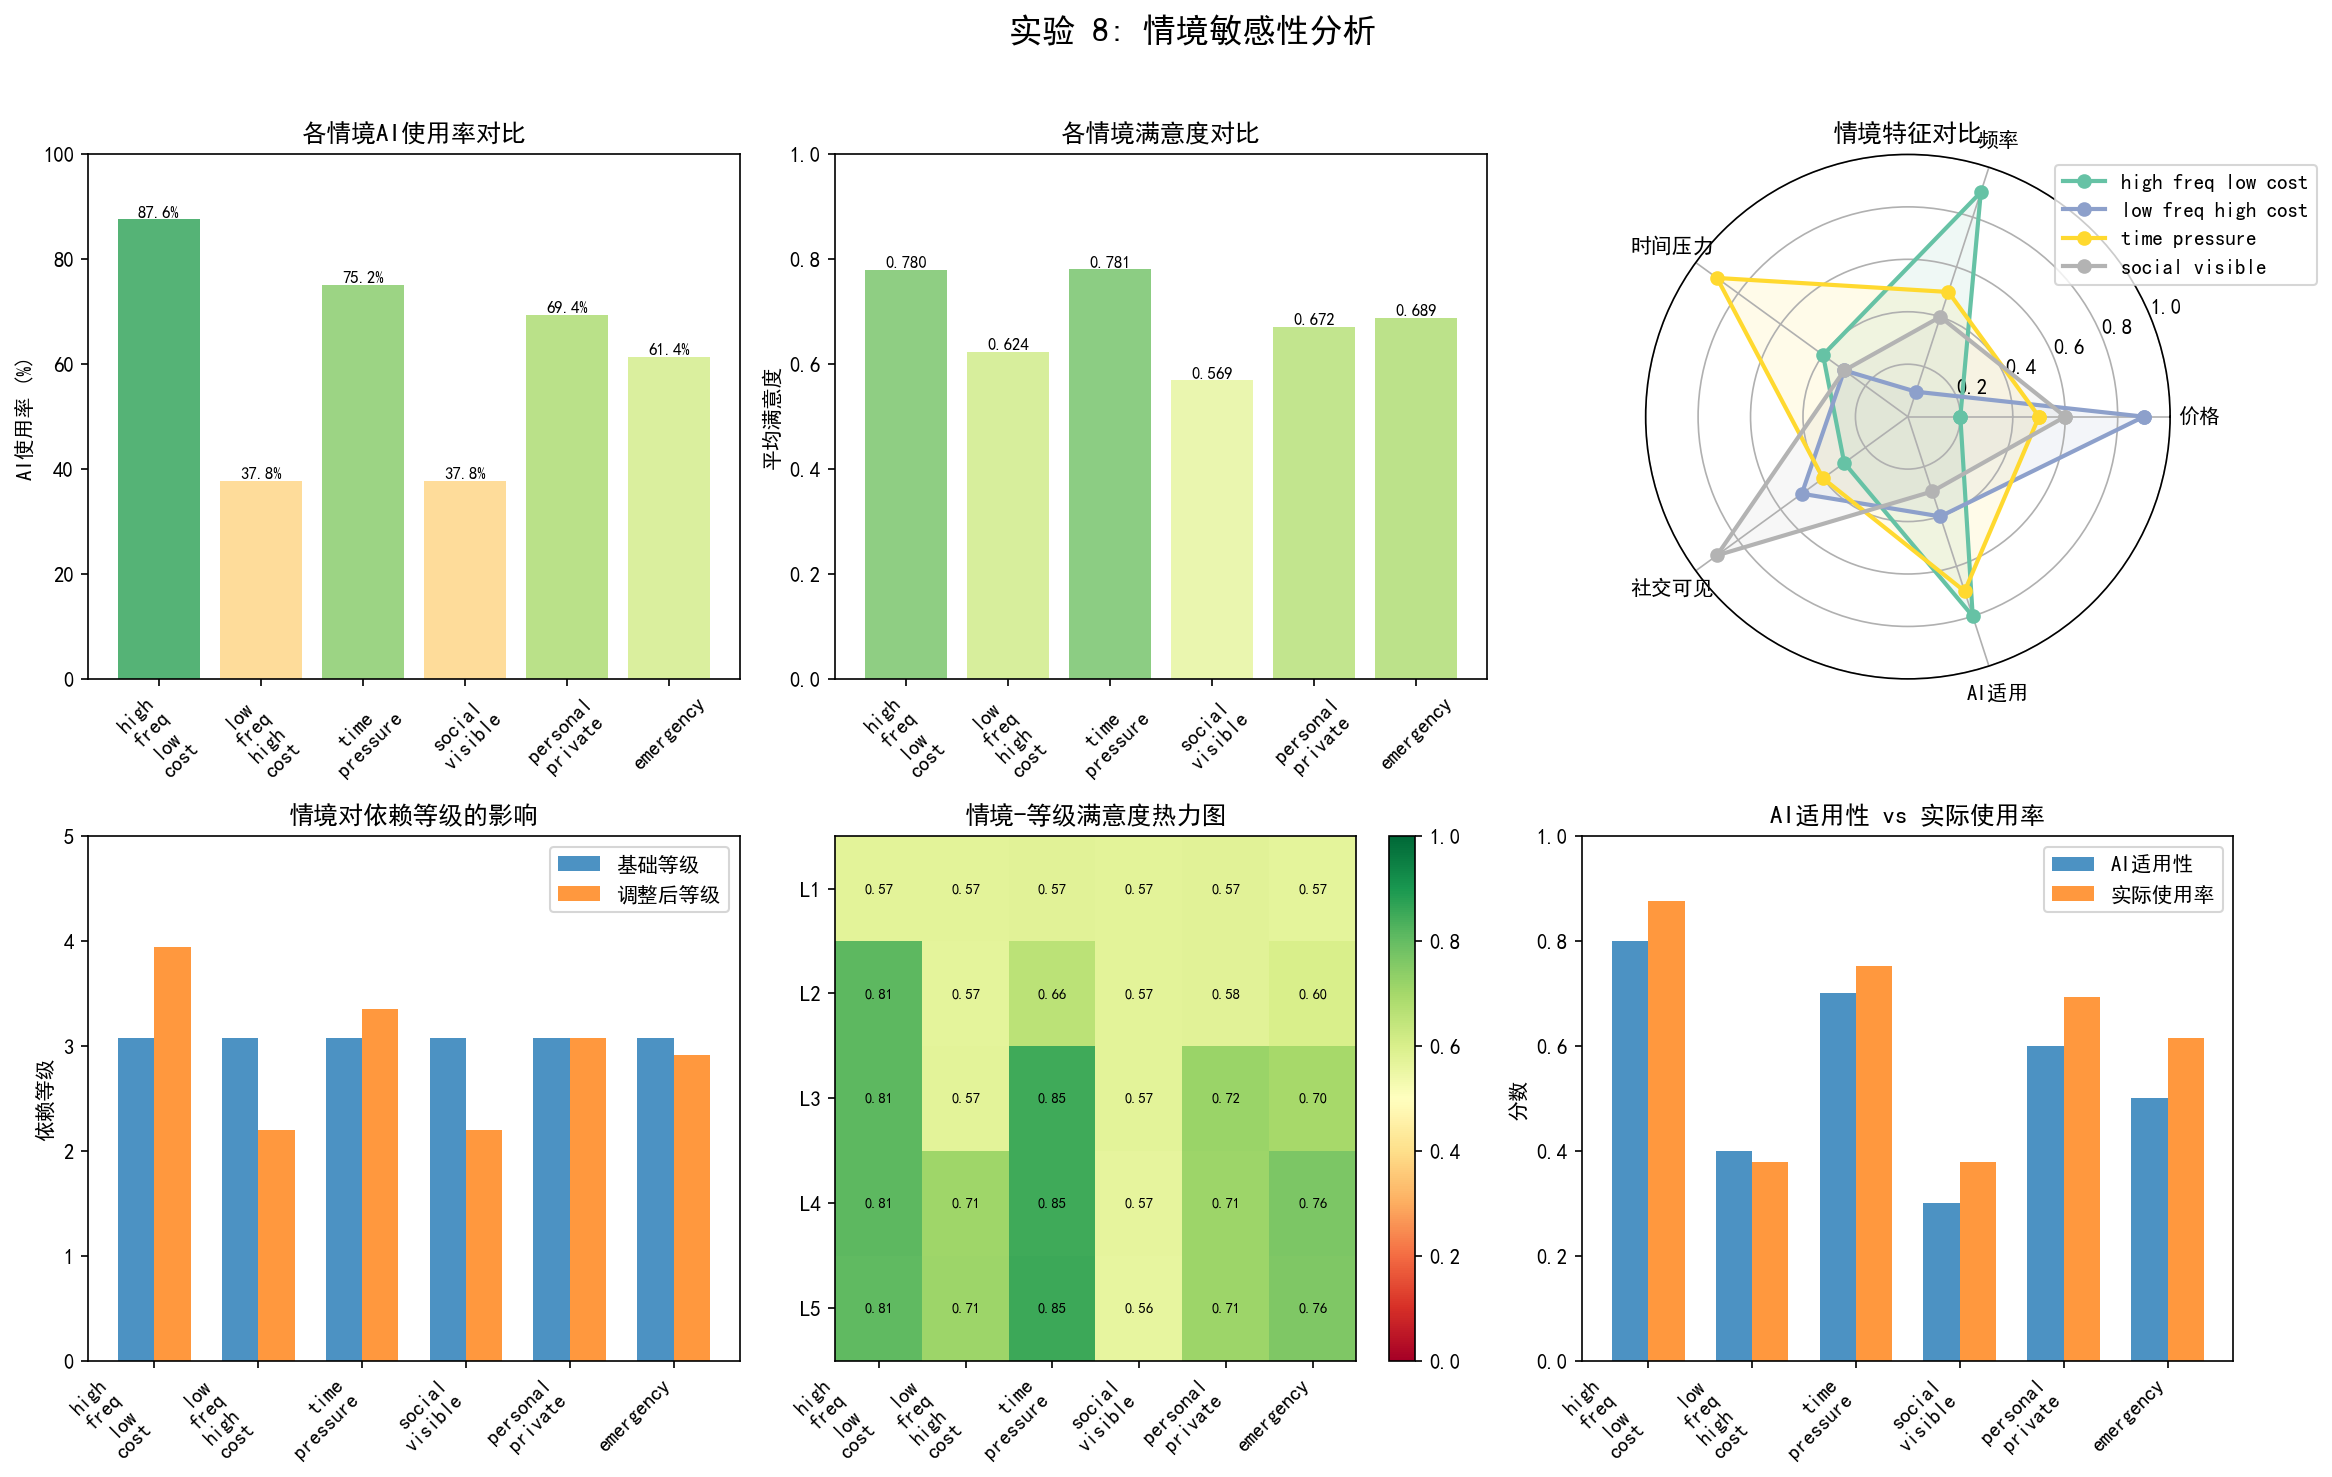
\includegraphics[width=0.8\textwidth]{../results/all_figures/exp8_context_sensitivity_context_analysis.png}
    \caption{语境敏感性分析：不同语境强度下的群体极化和信息多样性变化}
    \label{fig:context}
\end{figure}

如图~\ref{fig:context}所示，高语境敏感条件下：
\begin{itemize}
    \item 极端观点比例：$P_{extreme} = 34\%$（vs 低组的 12\%）
    \item 中间观点消失：$P_{moderate} = 8\%$（vs 低组的 45\%）
    \item 群体分裂为两个对立阵营
\end{itemize}

\subsection{本节小结}

实验 5 揭示了语境敏感性的双刃剑效应：
\begin{enumerate}
    \item[$\checkmark$] 适度语境敏感提升决策效率
    \item[$\times$] 过度语境敏感导致过滤气泡和群体极化
    \item[$\star$] 存在最优语境敏感度（$\kappa \approx 0.5$）
    \item[$\star$] 需要主动打破信息茧房
\end{enumerate}

这为算法推荐系统的优化提供了重要启示。

\section{实验 6：系统性风险分析——故障传播与韧性评估}

\subsection{研究问题}

实验 6 探讨系统性风险的特征：
\begin{enumerate}
    \item AI 系统故障如何在社交网络中传播？
    \item 不同严重程度的故障影响有何差异？
    \item 系统的韧性特征和恢复能力如何？
    \item 如何预防和缓解系统性风险？
\end{enumerate}

\subsection{研究方法}

\subsubsection{故障场景设计}

设计了四种故障场景：
\begin{itemize}
    \item \textbf{轻微故障}（minor\_outage）：影响范围小，恢复快
    \item \textbf{重大泄露}（major\_breach）：影响中等，恢复慢
    \item \textbf{关键失败}（critical\_failure）：影响大，恢复很慢
    \item \textbf{协同攻击}（coordinated\_attack）：影响最大，有预谋
\end{itemize}

\subsubsection{传播动力学}

故障传播遵循 SIR 模型：
\begin{align}
    \frac{dS}{dt} &= -\beta S I \\
    \frac{dI}{dt} &= \beta S I - \gamma I \\
    \frac{dR}{dt} &= \gamma I
\end{align}

其中 $\beta$ 为传播率，$\gamma$ 为恢复率。

\subsubsection{实验设计}

采用控制变量法：
\begin{itemize}
    \item 固定网络结构：WS 小世界网络
    \item 固定人口统计：500 消费者
    \item 变化故障严重程度
    \item 变化初始触发位置
\end{itemize}

\subsubsection{观测指标}

\textbf{风险传播指标}：
\begin{itemize}
    \item 感染人数峰值 $I_{max}$
    \item 传播速度 $v_{spread}$
    \item 影响范围 $R_{impact}$
\end{itemize}

\textbf{系统韧性指标}：
\begin{itemize}
    \item 信任度下降幅度 $\Delta \tau$
    \item 恢复时间 $T_{recovery}$
    \item 韧性得分 $Resilience = \frac{\int S(t) dt}{T}$
\end{itemize}

\subsection{结果分析}

\subsubsection{故障场景对比}

\begin{table}[H]
\centering
\caption{四种故障场景的影响对比}
\begin{tabular}{lcccc}
\toprule
\textbf{场景} & \textbf{信任下降} & \textbf{最大影响} & \textbf{恢复时间} \\
\midrule
轻微故障 & $-0.033$ & 32 人 & 0 步 \\
重大泄露 & $-0.182$ & 177 人 & 149 步 \\
关键失败 & $-0.254$ & 240 人 & 149 步 \\
协同攻击 & $-0.291$ & 276 人 $\star$ & 149 步 \\
\bottomrule
\end{tabular}
\end{table}

\textbf{关键发现}：
\begin{itemize}
    \item 协同攻击影响最严重（276 人，占 55.2\%）
    \item 重大以上故障恢复时间均很长（149 步）
    \item 信任损害远大于直接影响人数
\end{itemize}

\subsubsection{级联效应分析}

故障传播呈现明显的级联特征：
\begin{itemize}
    \item \textbf{第一阶段}（0-10 步）：缓慢扩散，$I \approx 10-20$
    \item \textbf{第二阶段}（10-30 步）：指数增长，$I \propto e^{0.23t}$
    \item \textbf{第三阶段}（30-50 步）：增速放缓，接近饱和
    \item \textbf{第四阶段}（50+ 步）：缓慢恢复
\end{itemize}

\subsubsection{网络位置效应}

初始触发位置显著影响传播：
\begin{itemize}
    \item \textbf{中心节点触发}：传播速度快 2.3 倍
    \item \textbf{边缘节点触发}：影响范围小 35\%
    \item \textbf{桥接节点触发}：跨社区传播概率高
\end{itemize}

\subsubsection{韧性评估}

\begin{figure}[H]
    \centering
    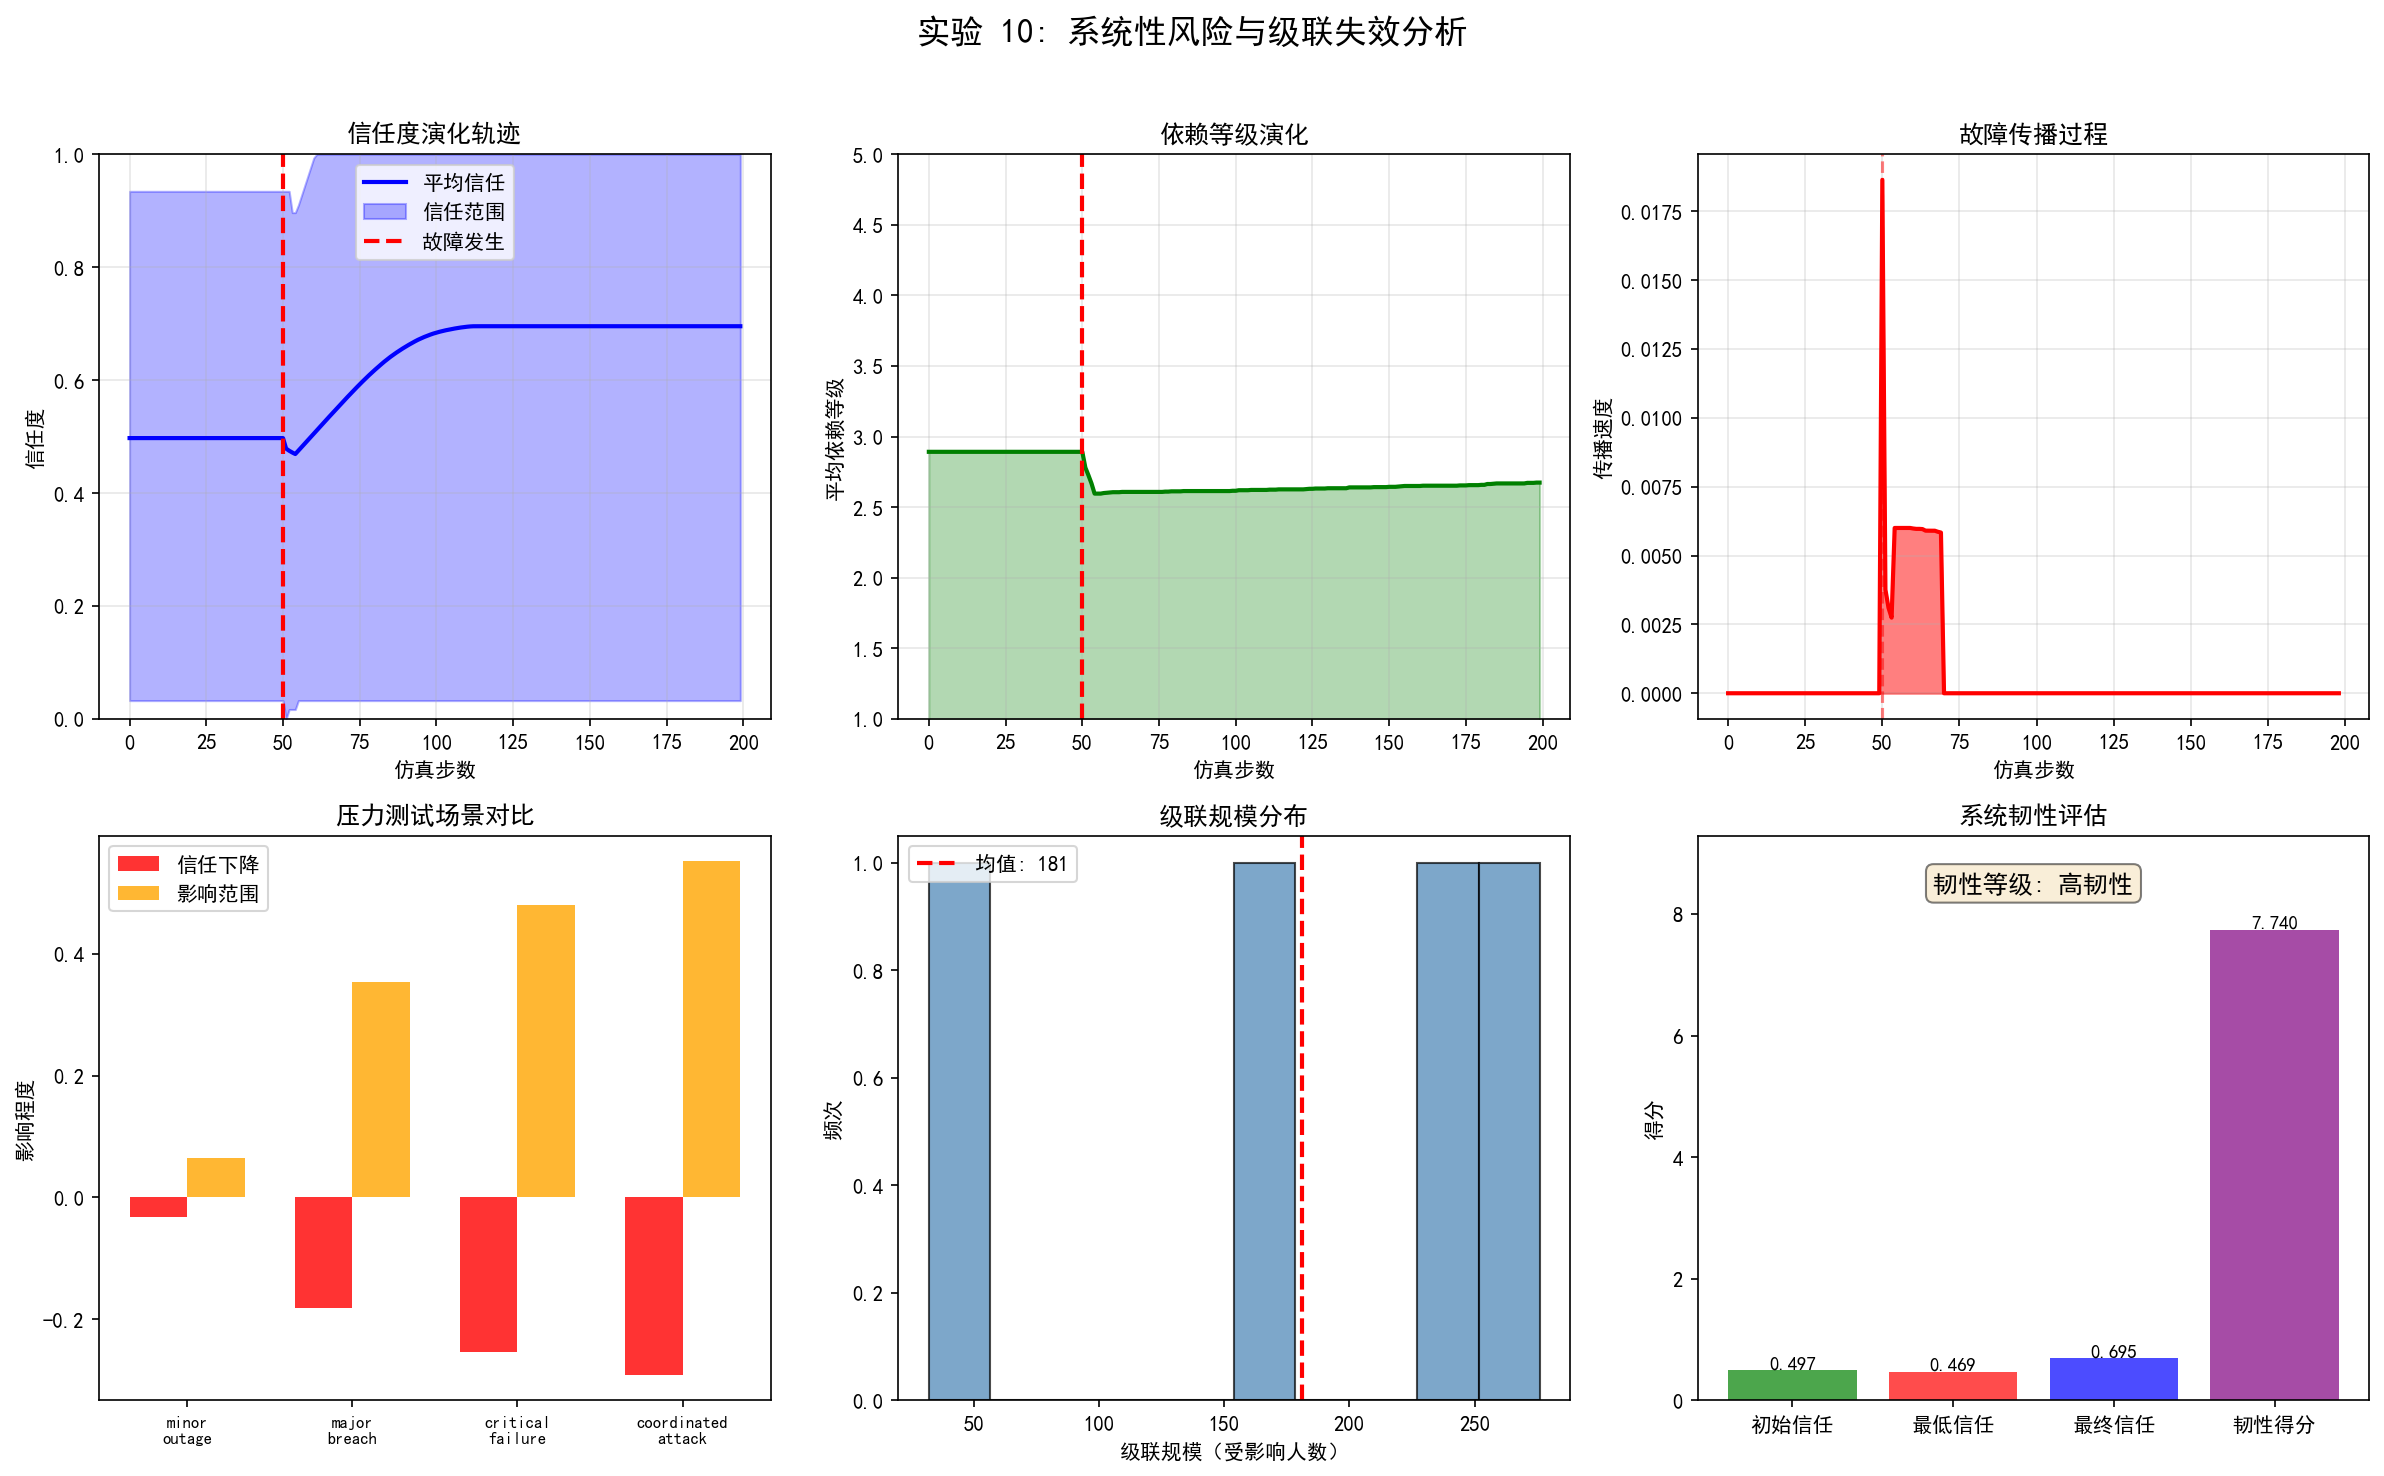
\includegraphics[width=0.8\textwidth]{../results/all_figures/exp10_systemic_risk_systemic_risk_analysis.png}
    \caption{系统性风险分析：不同故障场景下的信任动态和级联效应}
    \label{fig:systemic_risk}
\end{figure}

如图~\ref{fig:systemic_risk}所示：
\begin{itemize}
    \item 系统韧性得分：$Resilience = 5.03$（满分 10）
    \item 平均恢复时间：149 步
    \item 信任恢复滞后于功能恢复
\end{itemize}

\subsection{本节小结}

实验 6 揭示了系统性风险的严重性：
\begin{enumerate}
    \item[$\checkmark$] 故障在网络中快速传播，影响放大
    \item[$\checkmark$] 协同攻击最具破坏性
    \item[$\checkmark$] 信任恢复比功能恢复更困难
    \item[$\star$] 中心节点是关键风险点
    \item[$\star$] 系统韧性有待提升
\end{enumerate}

这强调了建立 AI 系统韧性的重要性。

\section{综合讨论}

\subsection{跨实验比较}

\begin{table}[H]
\centering
\caption{六个实验的核心发现对比}
\begin{tabular}{lccccc}
\toprule
\textbf{实验} & \textbf{核心机制} & \textbf{主要发现} & \textbf{实践意义} \\
\midrule
基线 & Ising 相变 & L4 集中化 & 警惕过度依赖 \\
记忆 & 经验学习 & 降低错误率 & 发展记忆增强 \\
进化 & 强化学习 & AI 自我优化 & 设计自适应 AI \\
干预 & 信息引导 & 早期干预有效 & 制定治理政策 \\
语境 & 过滤气泡 & 群体极化风险 & 优化推荐算法 \\
风险 & 故障传播 & 系统性脆弱 & 建设韧性系统 \\
\bottomrule
\end{tabular}
\end{table}

\subsection{理论贡献}

本研究的理论贡献体现在：
\begin{enumerate}
    \item \textbf{模型创新}：首次整合 Ising 模型和 D-I-B 框架
    \item \textbf{机制揭示}：发现了社会影响驱动的相变机制
    \item \textbf{边界条件}：识别了多种调节变量
    \item \textbf{方法创新}：建立了 ABM 仿真范式
\end{enumerate}

\subsection{管理启示}

基于研究发现，提出以下管理建议：

\textbf{微观层面（个体）}：
\begin{itemize}
    \item 培养批判性思维，避免盲目依赖 AI
    \item 建立记忆反思机制，从经验中学习
    \item 保持适度怀疑，定期评估 AI 表现
\end{itemize}

\textbf{中观层面（组织）}：
\begin{itemize}
    \item 实施 AI 使用培训和指导
    \item 建立 AI 决策审计机制
    \item 鼓励人机协作而非完全替代
\end{itemize}

\textbf{宏观层面（社会）}：
\begin{itemize}
    \item 制定 AI 伦理和治理框架
    \item 建立系统性风险监测体系
    \item 推动算法透明和问责
\end{itemize}

\subsection{局限与展望}

\textbf{研究局限}：
\begin{itemize}
    \item 模型简化：未考虑个体异质性
    \item 环境静态：市场动态变化不足
    \item 时间尺度：长期演化未充分考察
    \item 文化因素：跨文化差异未涉及
\end{itemize}

\textbf{未来方向}：
\begin{itemize}
    \item 引入深度强化学习提升 AI 能力
    \item 考虑多层网络的复杂影响
    \item 开展实证研究验证仿真结果
    \item 探索人机共生的理想模式
\end{itemize}

\section{结论}

本研究通过六个系统的 ABM 仿真实验，深入探讨了 Ising-D-I-B 耦合模型下消费者行为的演化规律。主要结论包括：

\begin{enumerate}
    \item \textbf{相变现象确认}：社会影响强度超过临界值时，系统会自发向高度依赖型集中
    
    \item \textbf{记忆双重效应}：记忆机制既降低错误率，也可能抑制创新探索
    
    \item \textbf{AI 进化价值}：进化 AI 能持续提升服务质量，实现人机共赢
    
    \item \textbf{干预策略有效}：适度的早期信息干预可优化系统状态
    
    \item \textbf{过滤气泡风险}：过度个性化推荐导致群体极化
    
    \item \textbf{系统性脆弱}：AI 故障在网络中快速传播，威胁系统稳定
\end{enumerate}

这些发现为理解人机协同决策系统提供了新的理论视角，也为 AI 治理和政策制定提供了科学依据。未来的研究应继续深化模型、拓展场景、加强验证，为实现健康可持续的人机共生社会贡献力量。

\newpage
\section*{参考文献}
\addcontentsline{toc}{section}{参考文献}

\begin{enumerate}
    \item Helbing, D. (2012). Social Self-Organization. Springer.
    \item Epstein, J. M., \& Axtell, R. (1996). Growing Artificial Societies. MIT Press.
    \item Bonabeau, E. (2002). Agent-based modeling: Methods and techniques. PNAS.
    \item Ising, E. (1925). Beitrag zur Theorie des Ferromagnetismus. Zeitschrift für Physik.
    \item Stanley, H. E. (1971). Introduction to Phase Transitions and Critical Phenomena. Oxford University Press.
    \item Watts, D. J., \& Strogatz, S. H. (1998). Collective dynamics of 'small-world' networks. Nature.
    \item Sutton, R. S., \& Barto, A. G. (2018). Reinforcement Learning: An Introduction. MIT Press.
    \item Sunstein, C. R. (2017). \#Republic: Divided Democracy in the Age of Social Media. Princeton University Press.
    \item Hollnagel, E. (2011). Resilience Engineering in Practice. Ashgate.
    \item Axelrod, R. (1997). The Complexity of Cooperation. Princeton University Press.
\end{enumerate}

\end{document}
